\documentclass{article}
\usepackage[utf8]{inputenc}
\usepackage{graphicx}

\title{Cloud Atlas \\[1ex] \large An LstmEncoder for UHECR AirShowers}
\author{Gianluca Becuzzi, Lucia Papalini}
\date{July 2022}

\begin{document}

\maketitle

In this project, we propose an example of using deep learning techniques to predict features of UHECR 
(Ultra High Energy Cosmic Rays) Showers.
In particular, when this kind of cosmic ray enters the atmosphere, they produce a particle cascade 
that can be identified with a set of water-Cherenkov or scintillator ground-based detectors. We aim to train a neural network to predict the height at which the shower formed by feeding it with data on the triggers of such detectors.\\
The dataset on which we perform the training consists of a simulation of an Auger-like apparatus 
made of a 9x9 array of detectors. The dataset is given as 80 flattened 9x9 matrices, that correponding to the time series part of the record, and another (flattened) matrix
in which each entry is the time of first detected activity, relative to the most intense detector.
The overall shape of the array is thus (80 + 1, 81).

The first step is splitting the dataset into the different features: the whole project is based on a custom NumPy \textit{dtype} for storing event's attributes in a single (?) sorted by \textit{toa}, \textit{time\_series} and \textit{outcome}.\\
First sight of the dataset showed the need for data augmentation at high values of height, so we built the \textit{Augmentation} class to perform that: it consists of increasing the number of those data by applying rotations and symmetry-flips on the various matrices.\\
Another important class is \textit{DataFeeder}, and the principle method gives back a \textit{Sequence} 
with whom we fed the network. It is a way to only train once on each sample per epoch.\\
%ALLUNGARE IL SUCCO
The network we built is a Concatenation of an LSTM (Long Short Term Memory) network for the \textit{time series} and an Encoder network for the \textit{time of arrival}, as shown in Fig \ref{fig:network}, ended with a series of dense layers that gives back a continuous output for the height of the shower. We built a class for each net module and another class to call them together: \textit{LushlooNet}.\\
To ensure better performance from the network, we also wrote a module to perform the \textit{hyperparameters tuning}.
\begin{figure}
    \centering
    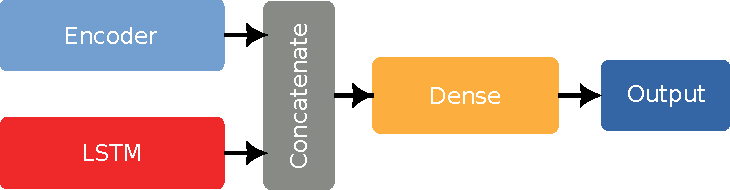
\includegraphics[width=0.9\textwidth]{figures/net_idea.pdf}
    \caption{}
    \label{fig:network}
\end{figure}




\end{document}